\documentclass[a4paper]{extarticle}

\usepackage[14pt]{extsizes}
\usepackage{comment}
\usepackage{enumitem}
\usepackage{hyperref}
\usepackage{cmap}
% \usepackage{tabu}
\usepackage{float}
\usepackage{mathptmx}
\usepackage{listings}
\usepackage{amsmath, amsfonts}
\usepackage{titlesec}
\usepackage{indentfirst}
\usepackage{graphicx}
\usepackage{longtable}
\usepackage[T2A]{fontenc}
\usepackage{mathtext}
\usepackage[utf8]{inputenc}
\usepackage[russian,english]{babel}

\renewcommand{\labelitemi}{–}
\renewcommand{\labelenumii}{\theenumii}
\renewcommand{\theenumii}{\theenumi.\arabic{enumii}.}
\setlist{nolistsep}

\setcounter{secnumdepth}{4}
\titleformat{\paragraph}
{\normalfont\normalsize\bfseries}{\theparagraph}{1em}{}
\titlespacing*{\paragraph}
{0pt}{3.25ex plus 1ex minus .2ex}{1.5ex plus .2ex}

\usepackage{chngcntr}
\counterwithin{figure}{section}
\counterwithin{table}{section}
\renewcommand{\thefigure}{\thesection.\arabic{figure}} % Формат рисунка секция.номер
\renewcommand{\thetable}{\thesection.\arabic{table}} % Формат таблицы секция.номер
\numberwithin{equation}{section}

\usepackage[tableposition=top]{caption}
\captionsetup[table]{
  labelsep = newline,
  textfont = sc, 
  name = TABLE, 
  justification=justified,
  singlelinecheck=false,
  labelsep=colon,
  skip = \medskipamount}
  
\usepackage{subcaption}
\DeclareCaptionLabelFormat{gostfigure}{Рисунок #2}
\DeclareCaptionLabelFormat{gosttable}{Таблица #2}
\DeclareCaptionLabelSeparator{gost}{~---~}
\captionsetup{labelsep=gost}
\captionsetup[figure]{labelformat=gostfigure}
\captionsetup[table]{labelformat=gosttable}
\renewcommand{\thesubfigure}{\asbuk{subfigure}}

\linespread{1.3}
\parindent=1.25cm
\setlist[enumerate,itemize]{itemindent=1.7cm, leftmargin=0cm}
\usepackage[left=20mm, top=15mm, right=15mm, bottom=15mm, nohead, footskip=10mm]{geometry}
\setlength{\parskip}{1.5pt}
\sloppy
\hyphenpenalty=10000
\clubpenalty=10000
\widowpenalty=10000
\setcounter{page}{7}

\lstset{
	basicstyle=\small\ttfamily,
    columns=fullflexible,
    breaklines=true,
}

\begin{document}

{\renewcommand{\contentsname}{Оглавление} \setlength{\parskip}{0cm} \tableofcontents \par}

\newpage
\section*{Введение}
\addcontentsline{toc}{section}{Введение}
В настоящее время большим спросом пользуются системы автоматизации деятельности различного вида предприятий. Представленные на рынке подобные системы весьма разнообразны.\par
В ряде субъектов Российской Федерации органами государственной власти используются продукты, построенные на программном комплексе "Web-Исполнение бюджета", реализованной предприятием "ООО "НПО Криста"[1]. Программный комплекс "Web-Исполнение Бюджета" предназначен для автоматизации деятельности органов государственной власти, органов местного самоуправления, государственных и муниципальных учреждений на всех этапах исполнения бюджета РФ. Программный комплекс позволяет организовать исполнение бюджета, обеспечивает ведения бюджетной отчетности и формирование аналитических форм отчетности.\par

\subsection*{Определения, обозначения и сокращения}
\addcontentsline{toc}{subsection}{Определения, обозначения и сокращения}
\begin{table}[H]
% \caption{Сокращения}
  \begin{tabular}{|c|c|c|}
  \multicolumn{3}{l}{Таблица 1 - Сокращения} \\
  \hline
  №  & Сокращение & Расшифровка \\\hline
  1  & ТЗ   & Техническое задание \\\hline
  2  & UML  & Unified Modeling Language \\\hline
  3  & JSON & JavaScript Object Notation \\\hline
  4  & XML  & Extensible Markup Language \\\hline
  5  & JVM  & Java Virtual Machine \\\hline
  6  & JDK  & Java SE Development Kit \\\hline
  7  & D3   & Data-Driven Documents \\\hline
  8  & SVG  & Scalable Vector Graphics \\\hline
  9  & DOM  & Document Object Model \\\hline
  10 & API  & Application Programming Interface \\
  \hline
  \end{tabular}
\end{table}\par
Подсистема визуализации - это подсистема, обеспечивающая интеграцию в программный комплекс "Web-Исполнение Бюджета" и процесс создания объекта визуализации.\par
Компонент создания объекта визуализации - это компонент подсистемы, который обрабатывает входные данные и преобразовывает их в блок HTML-кода, представляющий собой объект визуализации.\par
Объект визуализации - это графическое представление аналитического отчета, диаграмма. Объект визуализации состоит из наименования визуализации, геометрических фигур (точек, линий, фигур различной формы и цвета) и легенды, подписи с использованием цвета, определяющей категорию данных на диаграмме. Так же в зависимости от типа диаграммы может содержать оси, подписи к ним и маркеры осей.\par
Программный комплекс "Web-Исполнение Бюджета" - это система, в которую предстоит интегрировать подсистему визуализации.\par
Метки осей на графике или диаграмме - это категории, которые задают положение конкретных значений в ряде данных.\par

\newpage
\section{Анализ предметной области}
В процессе развития деловой и научной коммуникации возникает проблема предоставления информации, понятной широкому кругу людей. В следствии роста документного потока возникает потребность сокращения текста, свертывания информации или данных в более компактную структуру, в улучшении наглядности и читаемости, целостности отображения смысла высказываний, компактного обобщения данных. Для этого используется способ, который позволяет донести информацию и данные посредством визуальных образов.\par
Визуализация в мире аналитики — это диаграммы, графики и таблицы, различные формы представления, которые отображают данные. Визуальное изображение информации обозначают термином "информационная графика" или "инфографика". Инфографика может быть представлена в различных формах. Это матрицы, карты, иллюстрации, графики, диаграммы. Последние делятся на диаграммы сравнения, структурные, карты визуализации процесса, времени и связей.\par
Основная цель инфографики - информирование. При этом часто данный инструмент выступает в качестве дополнения к текстовой информации, сокращает аналитические или информационные данные, заменяя их на визуализированную, содержит некоторые пояснения.\par
Программный комплекс "Web-Исполнение Бюджета" оперирует значительным объемом бюджетных данных, документов, на основании которых строятся аналитические отчеты, представляемые в табличном виде. В связи с тем, что документооборот продолжает расти, появляется потребность в сжатии, наглядном и доступном преставлении данных. Инфографика поможет решить эту проблему с помощью представления табличных аналитических данных в виде визуализации.\par

\subsection{Постановка задачи}
Программный комплекс "Web-Исполнение бюджета" оперирует значительным объемом бюджетных данных, документов, и отчетов по этим документам. Поэтому было принято решение создать подсистему построения визуализации аналитического отчета на основе данных сформированных из уже имеющегося аналитического источника. Аналитический источник представляет собой выборку данных из БД по определенным правилам, указанным на интерфейсе Аналитические источники данных. Данные должны быть преобразованы в определенный формат и переданы для построения визуализации компоненту визуализации, входящему в состоав подсистемы визуализации. Подсистема визуализации должна быть интегрирована в программный комплекс "Web-Исполнение бюджета", разрабатываемый предприятием.\par
Возможно графическое представление табличных данных в виде трех типов диаграмм:
\begin{itemize}
  \item столбчатая диаграмма;
  \item круговая диаграмма;
  \item график.
\end{itemize}\par

\subsection{Обзор аналогов}
Представляемая подсистема создана для узкоспециализированной задачи и использования только в рамках программного продукта "Web-Исполнение бюджета".\par
При изучении рынка специализированного ПО было выявлено, что аналогичные "Web-Исполнению бюджета" системы так же используют подобный функционал. В большинстве этих систем используются комерческие приложения крупных компаний, таких, как Microsoft, Oracle, cluvio и других.\par
Oracle Data Visualization Cloud Service, Microsoft Excel Online и cluvio - это платные коммерческие приложения, которые требуют не разовую оплату продукта, а распространяются по системе подписки.
\begin{longtable}[H]{|p{0.2\textwidth}|p{0.35\textwidth}|p{0.35\textwidth}|}
  \caption{Преимущества и недостатки аналогов}
  \label{tableAnalog} \\\hline
  Технология & Преимущества & Недостатки \\\hline
  Oracle Data Visualization Cloud Service &
  	-Облачный сервис
  &
  	-Поддерживает только базу Oracle
  \\
  \multicolumn{3}{l}{}\\\multicolumn{3}{l}{}\\
  \caption*{Окончание таблицы \ref{tableAnalog}} \\\hline
  Microsoft Excel Online &
  	-Облачный сервис
  &
  	-Работает только с форматом .xls и .xlsx \newline
    -Только стандартные пресеты системы Microsoft Excel
  \\\hline
  cluvio &
  	-Облачный сервис \newline
    -Большое количество пресетов для графиков и диаграмм
  &
  	-Платный сервис, распространяемый по системе подписки
  \\\hline
\end{longtable}\par

\newpage
\section{Программная документация}

\subsection{Техническое задание}	

\subsubsection{Общие сведения}

\paragraph{Полное наименование подсистемы и ее условное обозначение}
Разработка подсистемы визуализации аналитических отчетов в системе бюджетирования.

\paragraph{Перечень документов, на основании которых создается подсистема, кем и когда утверждены эти документы}
Основанием для разработки "Планировщик выполнения заданий по расписанию" являются следующие документы и нормативные акты:\par
Задание на дипломный проект (приказ № 500-04 от 30.11.2016)

\paragraph{Плановые сроки начала и окончания работы по созданию подсистемы}
Плановый срок начала работ по созданию "Планировщик выполнения заданий по расписанию" – 15 апреля 2017 года. Плановый срок окончания работ по созданию "Планировщик выполнения заданий по расписанию" – 15 июня 2017 года.

\paragraph{Порядок оформления и предъявления заказчику результатов работ по созданию подсистемы}
Подсистема представляется в виде части программного продукта "Web-Исполнение бюджета" и не может быть использована вне пределов этой системы.

\paragraph{Перечень нормативно-технических документов, методических материалов, использованных при разработке ТЗ}
При разработке автоматизированной системы и создании проектно-эксплуатационной документации Исполнитель должен руководствоваться требованиями следующих нормативных документов:
\begin{itemize}
  \item ГОСТ 19.201-78. ТЕХНИЧЕСКОЕ ЗАДАНИЕ. ТРЕБОВАНИЯ К СОДЕРЖАНИЮ И ОФОРМЛЕНИЮ;
  \item ГОСТ 34.201-89. Информационная технология. Комплекс стандартов на автоматизированные системы. Виды, комплексность и обозначение документов при создании автоматизированных систем;
  \item РД 50-34.698-90. Методические указания. Информационная технология. Комплекс стандартов на автоматизированные системы. Автоматизированные системы. Требования к содержанию документов.
\end{itemize}

\subsubsection{Назначение разработки}
Назначением подсистемы является предоставление пользователю возможности более эффективного анализа данных.

\subsubsection{Цель создания подсистемы}
Целью создания подсистемы визуализации отчета является возможность визуализации аналитических данных в web-браузере с использованием различных видов диаграмм. Совместимость с технической платформой автоматизированной системы "Web-Исполнение бюджета". Поддержка корректной работы в актуальных версиях браузеров Mozilla Firefox, Yandex Browser, Google Chrome.

\subsubsection{Требования к системе}

\paragraph{Требования к характеристикам взаимосвязей создаваемой системы со смежными системами}
Подсистема визуализации отчетов должен взаимодействовать со следующими интерфейсами программного комплекса "Web-Исполнения бюджета":\par
\begin{itemize}
  \item интерфейс создания и управления аналитическими источниками данных;
  \item интерфейс администрирования аналитических отчетов;
  \item интерфейс отображения аналитических отчетов.
\end{itemize}\par
Возможны следующие варианты взаимодействия с программным комплексом "Web-Исполнения бюджета":
\begin{itemize}
  \item создание аналитического источника данных на интерфейсе создания и управления аналитическими источниками данных;
  \item заполнение шаблона визуализации отчета пользовательскими параметрами;
  \item создание объекта визуализации посредством интерфейса\newline администрирования аналитических отчетов;
  \item прикрепление аналитического источника данных к элементу визуализации на интерфейсе администрирования аналитических отчетов;
  \item получение данных из шаблона визуалиации с пользовательскими параметрами и аналитического источника данных;
  \item отображение объекта визуализации внутри интерфейса отображения аналитических отчетов.
\end{itemize}

\paragraph{Требования к эргономике и технической эстетике}
Взаимодействие пользователя с web-интерфейсом подсистемы визуализации, входящим в состав программного комплекса "Web-Исполнение бюджета" должно осуществляться посредством визуального графического интерфейса (GUI). Внешний вид интерфейса подсистемы визуализации не должен отличаться от общего внешнего вида интерфейса всего программного комплекса.\par
Интерфейс должен быть рассчитан на преимущественное использование манипулятора типа "мышь", то есть управление системой должно осуществляться с помощью набора экранных меню, кнопок и т. п. элементов. Клавиатурный режим ввода должен используется главным образом при заполнении и/или редактировании текстовых и числовых полей экранных форм.\par
Все надписи экранных форм, а также сообщения, выдаваемые пользователю (кроме системных сообщений) должны быть на русском языке.

\paragraph{Требования к эксплуатации, техническому обслуживанию, ремонту и хранению компонентов системы}
Система должны быть рассчитана на эксплуатацию в составе программного комплекса "Web-Исполнение бюджета". Для нормальной эксплуатации разрабатываемой системы должно быть обеспечено бесперебойное питание ПЭВМ.\par
Периодическое техническое обслуживание используемых ПК должно проводиться не реже одного раза в год.\par
При вводе системы в опытную эксплуатацию должен быть разработан план резервного копирования программного обеспечения и обрабатываемой информации. Во время эксплуатации системы, персонал, ответственный за эксплуатацию системы должен выполнять разработанный план.\par
Квалификация персонала и его подготовка должны соответствовать документации.

\paragraph{Требования к патентной чистоте}
Подсистема входит в состав "Web-Исполнение Бюджета", поэтому для использования необходима лицензионная версия этого программного продукта.

\paragraph{Требования к численности и квалификации персонала}
Для обслуживания модуля требуется один программист с базовыми знаниями языков программирования JavaScript, Java и понимающий внутреннее устройство программного комплекса "Web-Исполнение Бюджета".

\paragraph{Требования к режиму работы персонала}
Система реализуется на персональных компьютерах, поэтому требования к режиму отдыха и организации труда при работе с ней должны устанавливаться, исходя из требований к организации труда и режима отдыха при работе с этим типом средств вычислительной техники.\par
Для обеспечения максимальной работоспособности и сохранения здоровья профессиональных пользователей на протяжении рабочей смены должны устанавливаться регламентированные перерывы: через 2 часа после начала рабочей смены и через 1,5 – 2,0 часа после обеденного перерыва продолжительностью 15 минут каждый или продолжительностью 10 минут через каждый час работы.\par
Продолжительность непрерывной работы персонала с разрабатываемой системой и персональными компьютерами без регламентированного перерыва не должна превышать 2 часа.\par
Деятельность персонала по эксплуатации системы должна регулироваться должностными инструкциями.

\paragraph{Требования к надежности}
Система должна сохранять работоспособность и обеспечивать восстановление своих функций при возникновении следующих внештатных ситуаций:\par
\begin{itemize}
	\item при сбоях в системе электроснабжения аппаратной части, приводящих к перезагрузке ОС, восстановление программы должно происходить после перезапуска ОС и запуска исполняемого файла системы;
	\item при ошибках в работе аппаратных средств (кроме носителей данных и программ) восстановление функции системы возлагается на ОС;
	\item при ошибках, связанных с программным обеспечением (ОС и драйверы устройств), восстановление работоспособности возлагается на ОС.\par
\end{itemize}\par
Для защиты аппаратуры от бросков напряжения и коммутационных помех должны применяться сетевые фильтры.

\subsubsection{Требования к функциям, выполняемым системой}
Подсистема визуализации аналитического отчета должна обеспечивать следующую функциональность:\par
\begin{itemize}
  \item возможность преобразовывать аналитический источник данных в удобный для передачи и чтения компонентом визуализации формат;
  \item возможность запрашивать у пользователя параметры визуализации (наименование визуализации, названия осей, тип визуализации);
  \item возможность объединения собранных данных в удобный для передачи и чтения компонентом визуализации формат;
  \item возможность построения объекта визуализации, который должен содержать:\newline
    	\hspace*{2.5cm} – наименование визуализации;\newline
        \hspace*{2.5cm} – легенду, указывающую описание к маркерам данных;\newline
    	\hspace*{2.5cm} – оси и подписи к ним;\newline
        \hspace*{2.5cm} – метки осей;
  \item возможность интеграции объекта визуализации в программный комплекс "Web-Исполнение бюджета".
\end{itemize}\par
Работа подсистемы предусматривает непрерывную круглосуточную работу и доступность сервисов программного продукта "Web-Исполнение бюджета" в режиме 24х7х365 (с учетом перерывов на техническое обслуживание).

\paragraph{Требования к организации входных данных}
Для компонента визуализации, который будет формировать непосредственно объект визуализации, требуется сформировать входные данные. Входными данными для компонента визуализации должен быть объект в удобном для передачи и чтения компонентом визуализации формате, сформированный после обработки аналитического источника данных и установленных пользователем параметров. Он должен включать в себя:\par
\begin{itemize}
  \item тип отображаемой диаграммы (столбчатая, круговая, график);
  \item заголовок отображаемой диаграммы (по умолчанию идентичен наименованию аналитического источника);
  \item названия осей диаграммы;
  \item JSON–массив данных, представляющий из себя набор (выборку) данных для конкретного вида диаграммы.
\end{itemize}\par
Вид входных данных:\par
\lstset{inputencoding=utf8, extendedchars=\true, commentstyle=\itshape}
\begin{lstlisting}[language=Java]
[{
	"type": "Тип выводимой диаграммы",
	"caption": "Заголовок диаграммы",
	"x_name": "Наименование оси X",
	"y_name": "Наименование оси Y",
	"data":[{"x": "данные по оси x", "y": "данные по оси y"},]
}]
\end{lstlisting}

\paragraph{Требования к организации выходных данных}
Выходными данными компонента визуализации должен быть блок HTML-кода, представляющий из себя графическое представление , диаграмму с интерактивными функциями взаимодействия:
\begin{itemize}
  \item выделение столбца (если столбчатая диаграмма) или части диаграммы (если круговая диаграмма) при наведении;
  \item всплывающая подсказка с дополнительной информацией при наведении на столбец или часть круговой диаграммы.
\end{itemize}

\subsubsection{Требования к видам обеспечения}

\paragraph{Требования к составу и параметрам технических средств сервера системы}
Требования к аппаратной части[1]:\par
\begin{itemize}
  \item серверный процессор - не менее 4 физических ядер;
  \item оперативная память - не менее 24 Гб;
  \item подсистема хранения данных для системы, СУБД, файлов СУБД - не мене 100 Гб в год, рекомендуется RAID 10;
  \item подсистема резервного хранения данных - от 1 Тб (общая с сервером приложений); резервирование питания.
\end{itemize}\par
Требования к каналам связи: между сервером приложений и сервером БД не менее 1 Гбит/с.\par
Требования к программному обеспечению:\par
\begin{itemize}
  \item операционная система: Ubuntu Server 14.04 LTS;
  \item СУБД: PostgreSQL.
\end{itemize}\par

\paragraph{Требования к составу и параметрам технических средств рабочего места пользователя}
Разрабатываемое программное обеспечение должно функционировать в операционных системах Windows XP(32-bit) / Vista (32- или 64-bit) / Windows 7 (32- или 64-bit).\par
Минимальные требования к техническим характеристикам ПК пользователя[1]:\par
\begin{itemize}
  \item процессор с тактовой частотой не ниже 800 МГц;
  \item объем оперативной памяти (RAM): 4 Гб;
  \item дисковая подсистема с объемом свободной памяти не менее 20 Гб.
\end{itemize}\par
Требования к каналам связи между клиентским устройством и сервером:\par
\begin{itemize}
  \item время прохождения пакета (ping) от клиента до сервера не больше 100 мс;
  \item скорость передачи данных: от 256 Кбит/с при однопользовательской работе, от 1024 Кбит/с для 2-4 пользователей.
\end{itemize}

\paragraph{Требования к программному обеспечению}
Актуальная версия браузера Mozilla Firefox, Yandex Browser или Google Chrome (с поддержкой версии JavaScript ECMAScript 6 и старше[8]). JavaScript-библиотека jQuery версии 3.1 и старше. JavaScript-библиотека D3.js версии 4.8.0 и старше. При использовании ЭП - криптографическое ПО.

\paragraph{Требования к документации на дипломный проект}
В состав документации на дипломный проект входят следующие разделы и документы:\par
Введение\par
\qquad Определения, обозначения и сокращения\par
1.	Анализ предметной области\par
\qquad 1.1.	Постановка задачи\par
\qquad 1.2.	Обзор аналогов\par
2.	Техническое задание\par
3.	Пояснительная записка\par
4.	Описание программы\par
5.	Программа и методика испытаний\par
6.	Эксплуатационная документация (Руководство оператора)\par
7.	Акт испытаний программного продукта\par
8.	Экономическая часть\par
Заключение\par
Список литературы\par
Приложения\par

\subsection{Пояснительная записка}

\subsubsection*{Введение}
\addcontentsline{toc}{subsubsection}{Введение}
Наименование разрабатываемой системы приводится в техническом задании, раздел "2.1.1 Полное наименование системы и ее условное обозначение".\par
Документы, на основании которых ведется проектирование, приводятся в техническом задании, раздел "2.1.2 Перечень документов, на основании которых создается система".\par
Стадии и сроки исполнения приведены в техническом задании, раздел "2.1.3 Плановые сроки начала и окончания работы по созданию системы".

\subsubsection{Назначение и области применения}
Подсистема визуализации аналитических отчетов обеспечивает создание различных диаграмм. Подсистема используется в системах бизнес-аналитики и предназначена для повышения эффективности и для осуществления более качественного анализа большого количества аналитических данных.

\subsubsection{Технические характеристики}

\paragraph{Постановка задачи на разработку подсистемы}
Анализ предметной области выявил необходимость внедрения в программный комплекс "Web-Исполнение бюджета" подсистемы визуализации табличных отчетов, построенных на основе аналитических источников данных.\par
Разрабатываемая подсистема должна решать следующие задачи:
\begin{itemize}
  \item обрабатывать и преобразовывать аналитический источник данных в специальный формат;
  \item запрашивать у пользователя параметры визуализации (наименование визуализации, названия осей, тип визуализации);
  \item объединять собранные данных в удобный для передачи и чтения компонентом визуализации формат;
  \item строить объект визуализации;
  \item интегрировать объект визуализации в программный комплекс "Web-Исполнение бюджета".
\end{itemize}\par

\paragraph{Описание общей структурной схемы и функционирования подсистемы}
Подсистема визуализации встраивается в программный комплекс\newline "Web-Исполнение бюджета". Работа с подсистемой происходит в несколько этапов:\par
\begin{itemize}
	\item Для начала необходимо создать Аналитический источник данных.\par
  Создание аналитического источника начинается с выбора Идентификатора данных - это модель данных, из которой будет происходить выборка данных. Затем в новый аналитический источник добавляются колонки из модели данных, которые будут использоваться при формировании данных для отчета. После добавления колонок требуется написать события, которые будут отвечать за содержание данных во время подготовки параметров (событие На подготовку параметров), после закачки данных (событие После закачки) после формирования данных.
	\item Далее создается шаблон визуализации в формате .template. Это делается на интерфейсе Администратор отчетов.
  Созданный шаблон можно редактировать на том же интерфейса в Редакторе шаблонов, где можно выбрать наименование диаграммы, наличие на диаграмме легенды и вид диаграммы.
    \item Следующим этапом будет создание нового объекта визуализации на интерфейсе Администратор отчетов. Там выбираются шаблон, источник данных, на основании которых будет строится визуализация и указываются нужные параметры визуализации.
    \item После создания объекта визуализации его можно выполнить на интерфейсе Отчеты. Как и на интерфейса Администратор отчетов, здесь можно править шаблон визуализации с помощью Редактора шаблонов.
\end{itemize}\par
Диаграммы вариантов использования подсистемы построения аналитических отчетов до внедрения подсистемы визуализации аналитических отчетов и после ее внедрения представлены на рисунке (Рисунок \ref{ris2}).
\begin{figure}[H]
\center{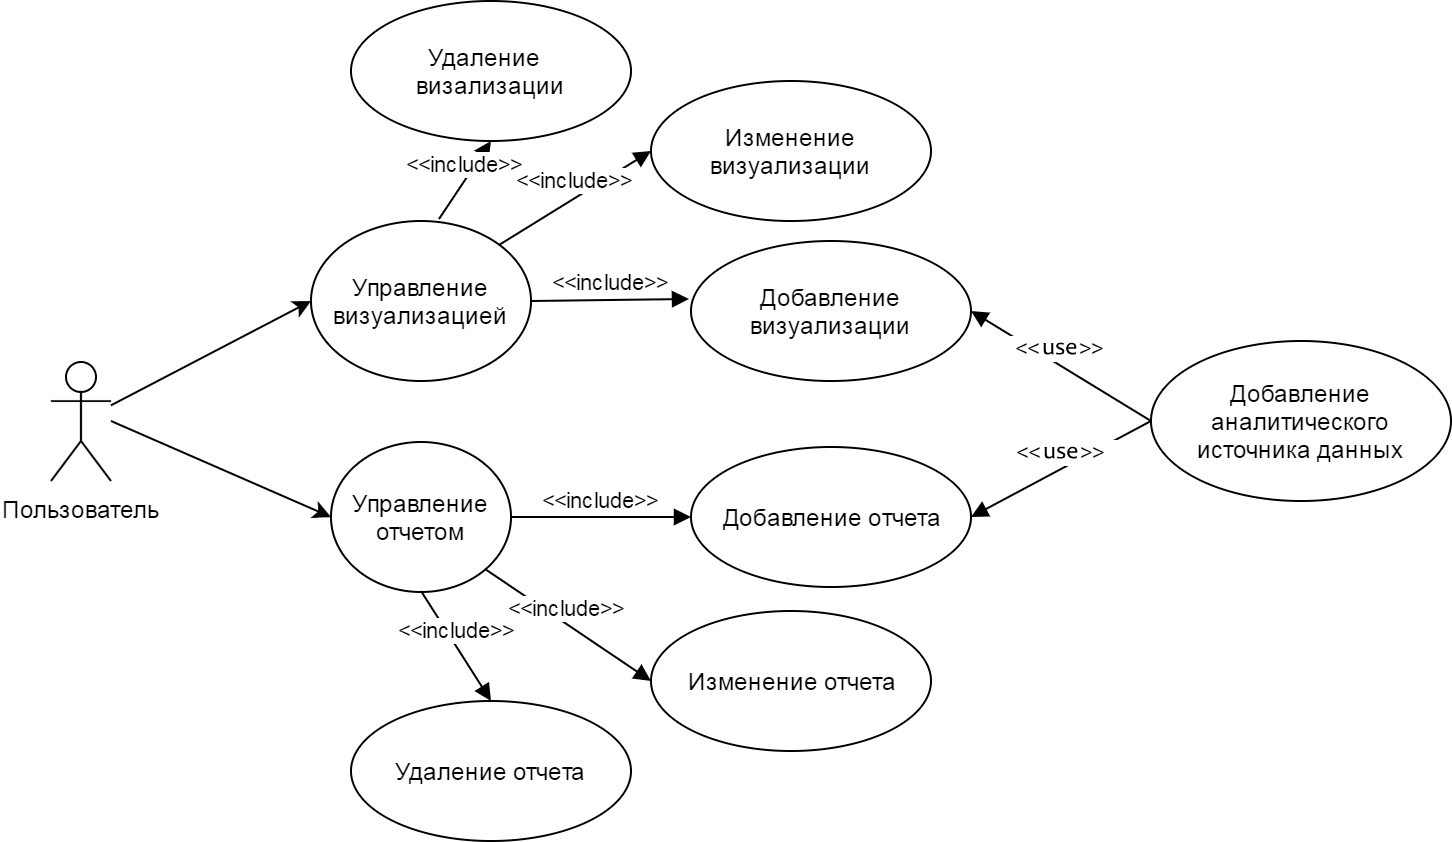
\includegraphics[width=17cm]{./imgs/2.png}}
\centering
\caption{Схема бизнес-логики разрабатываемой подсистемы}
\label{ris2}
\end{figure}\par

\paragraph{Описание и обоснование выбора метода организация входных и выходных данных}
Входные данные представлены в виде JSON-объекта, который содержит данные из шаблона визуализации, параметры заданные на интерфейсе Администратор отчетов и данных из Аналитического источника. Выбор формата JSON обусловлен следующим:
\begin{itemize}
\item При написании компонента визуализации предполагается использовать JavaScript, а JSON - это текстовый формат основанный на JavaScript[8];
\item Формат JSON удобнее обрабатывать языком JavaScript, в отличие от других форматов передачи данных.
% \begin{table}[H]
% \caption{Сравнениек разбора JSON, XML и YAML объектов на языке JavaScript.}
% \centering
%   \begin{tabular}{|c|c|c|c|}
%   \hline
%   Формат & Содержание & Разбор \\\hline
%   JSON  &  
%   %картинка с JSON
%   & 
%   %картинка с кодом парсинга JSON
%   \\\hline
%   XML   &  
%   %картинка с XML
%   & 
%   %картинка с кодом парсинга XML
%   \\\hline
%   YAML  & 
%   %картинка с YAML
%   & 
%   %картинка с кодом парсинга YAML
%   \\\hline
%   \end{tabular}
% \end{table}\par
\end{itemize}

\paragraph{Описание и обоснование выбора состава технических и программных средств}
Для написания компонентов интеграции подсистемы визуализации аналитических отчетов в программный комплекс "Web-Исполнение бюджета" использован язык Java[5], а в качестве языка для написания клиентских и серверных скриптов использован язык JavaScript. Обосновано это тем, что программный комплекс "Web-Исполнение бюджета" является web-приложением, серверная часть которого написана на языке Java, а все взаимодействие JavaScript и HTML на стороне клиента происходит с помощью JavaScript-библиотеки jQuery.\par
В качестве инструмента для написания компонента создания объекта визуализации используется JavaScript-библиотека D3.js. D3.js – это самый низкоуровневый инструмент для работы с языком разметки svg[3]. Библиотека, в отличие от своих многочисленных аналогов, объединяет работу с SVG (базисом для работы с этим языком разметки является SVG API), CSS и DOM моделью, что является большим плюсом для программного комплекса "Web-Исполнение бюджета", которое является web-приложением. В отличие от своих аналогов библиотека предоставляет синтаксис схожий с синтаксисом JavaScript-библиотеки jQuery, что актуально для программного комплекса "Web-Исполнение бюджета", являющимся web-приложением. Большинство библиотек визуализации предоставляют готовые шаблоны для визуализации и не дают гибкого инструмента для построения своих шаблонов. D3.JS не имеет готовых реализаций шаблонов, но у нее есть огромная библиотека с примерами, написанными с ее помощью.\par
Таким образом D3.JS была выбрана в качестве основного средства построения визуализации в подсистеме.

\subsection{Описание программы}

\subsubsection{Общие сведения}
Пользователь имеет возможность создания визуализации аналитического отчета на основе заранее сформированного разработчиком аналитического источника данных и настроенного им же объекта визуализации.\par
Технология создания аналитического источника данных выглядит в виде таблицы, в которой разработчику предоставляется возможность установить наименование аналитического источника, написать события на языке JavaScript, которые будут отвечать за содержание данных во время подготовки параметров (событие На подготовку параметров), после закачки данных (событие После закачки) после формирования данных. В детализации требуется указать секции, из которых будут выкачиваться данные и колонки, то есть какие именно данные будут обрабатываться событиями.\par
После создания аналитического источника разработчику необходимо создать шаблон и объект визуализации. Технология создания шаблона выглядит в виде модального окна, где задаются параметры будущей визуализации, такие как:
\begin{itemize}
  \item наименование диаграммы;
  \item флаг указывающий наличие на диаграмме легенды;
  \item наименования осей диаграммы;
  \item вид диаграммы.
\end{itemize}\par
Когда шаблон визуализации заполнен и сохранен требуется создать непосредственно объект визуализации. Для этого разработчику нужно выбрать и заполнить номер отчет, который будет содержать комбинацию групп цифр относящих его к определенной группе, наименование отчета, выбрать из списка шаблонов созданный ранее шаблон визуализации, так же выбрать формат отчета, то есть, в нашем случае, диаграмму (d3\_diagram) и выставить флаг использования (или снять флаг для внесения изменений в объект визуализации. Детализация содержит форму добавления аналитического источника данных из списка существующих и форму добавления пользовательских параметров для передачи механизму построения аналитического отчета или подсистеме визуализации аналитических отчетов.\par
Когда пользователь запускает процесс построения визуализации, в действие приводятся написанные разработчиком события, формирующие аналитические данные, выбираются пользовательские параметры объекта аналитичекого отчета и параметры из шаблона визуализации. После того, как аналитические данные полностью сформировались, они формируются в JSON-объект вместе с пользовательскими параметрами объекта аналитичекого отчета и параметрами из шаблона визуализации и передаются компоненте построения визуализации.

\paragraph{Программное обеспечение, необходимое для функционирования программы}
Для функционирования подсистемы необходима актуальная версия браузера Mozilla Firefox, Yandex Browser или Google Chrome (с поддержкой версии JavaScript ECMAScript 6 и старше[8]). При использовании ЭП – криптографическое ПО.

\paragraph{Используемые при разработке языки программирования и инструментальные средства}
Java – объектно–ориентированный структурный императивный язык программирования со строгой полиморфной статической явной системой типов. Программы на Java транслируются в байт-код, что делает их практически не зависимыми от операционной системы.\par
JavaScript – это скриптовый язык, предназначенный для создания интерактивных веб-страниц. Его не требуется компилировать, он подключается к HTML-странице и работает "как есть". JavaScript обычно используется как встраиваемый язык для программного доступа к объектам приложений. Наиболее широкое применение находит в браузерах как язык сценариев для придания интерактивности веб-страницам.\par
В качестве СУБД применяется PostgreSQL. Для организации версионного хранилища используется система контроля версий Mercurial (Hg) и TortoiseHg в качестве графического фронтенда.\par
Для визуализации табличного аналитического отчета, то есть построения диаграммы была использована JavaScript библиотека D3.js.\par
D3.js (название D3 расшифровывается как data driven document) - это JavaScript-библиотека для обработки и визуализации данных. Она предоставляет удобные утилиты для обработки и загрузки массивов данных и создания DOM-элементов[3].

\subsubsection{Функциональное назначение}
Функциональные возможности подсистемы визуализации аналитического отчета:\par
\begin{itemize}
  \item возможность преобразовывать аналитический источник данных в удобный для передачи и чтения компонентом визуализации формат;
  \item возможность запрашивать у пользователя параметры визуализации (наименование визуализации, названия осей, тип визуализации);
  \item возможность объединения собранных данных в удобный для передачи и чтения компонентом визуализации формат;
  \item возможность построения объекта визуализации, который должен содержать:
    \begin{itemize}
    	\item наименование визуализации;
        \item легенду, указывающую описание к маркерам данных;
    	\item оси и подписи к ним, если выбрана столбчатая диаграмма или график;
        \item метки осей - категории, которые задают положение конкретных значений в ряде данных;
    \end{itemize}
  \item возможность интеграции объекта визуализации в программный комплекс "Web-Исполнение бюджета".
\end{itemize}\par

\subsubsection{Структура программы (модули, классы)}
Структура разработанной подсистемы[8] визуализации аналитических источников представленна на рисунках (Рисунок \ref{umlClassDiagram:ris1} и Рисунок \ref{umlClassDiagram:ris2}).
\begin{figure}[H]
\center{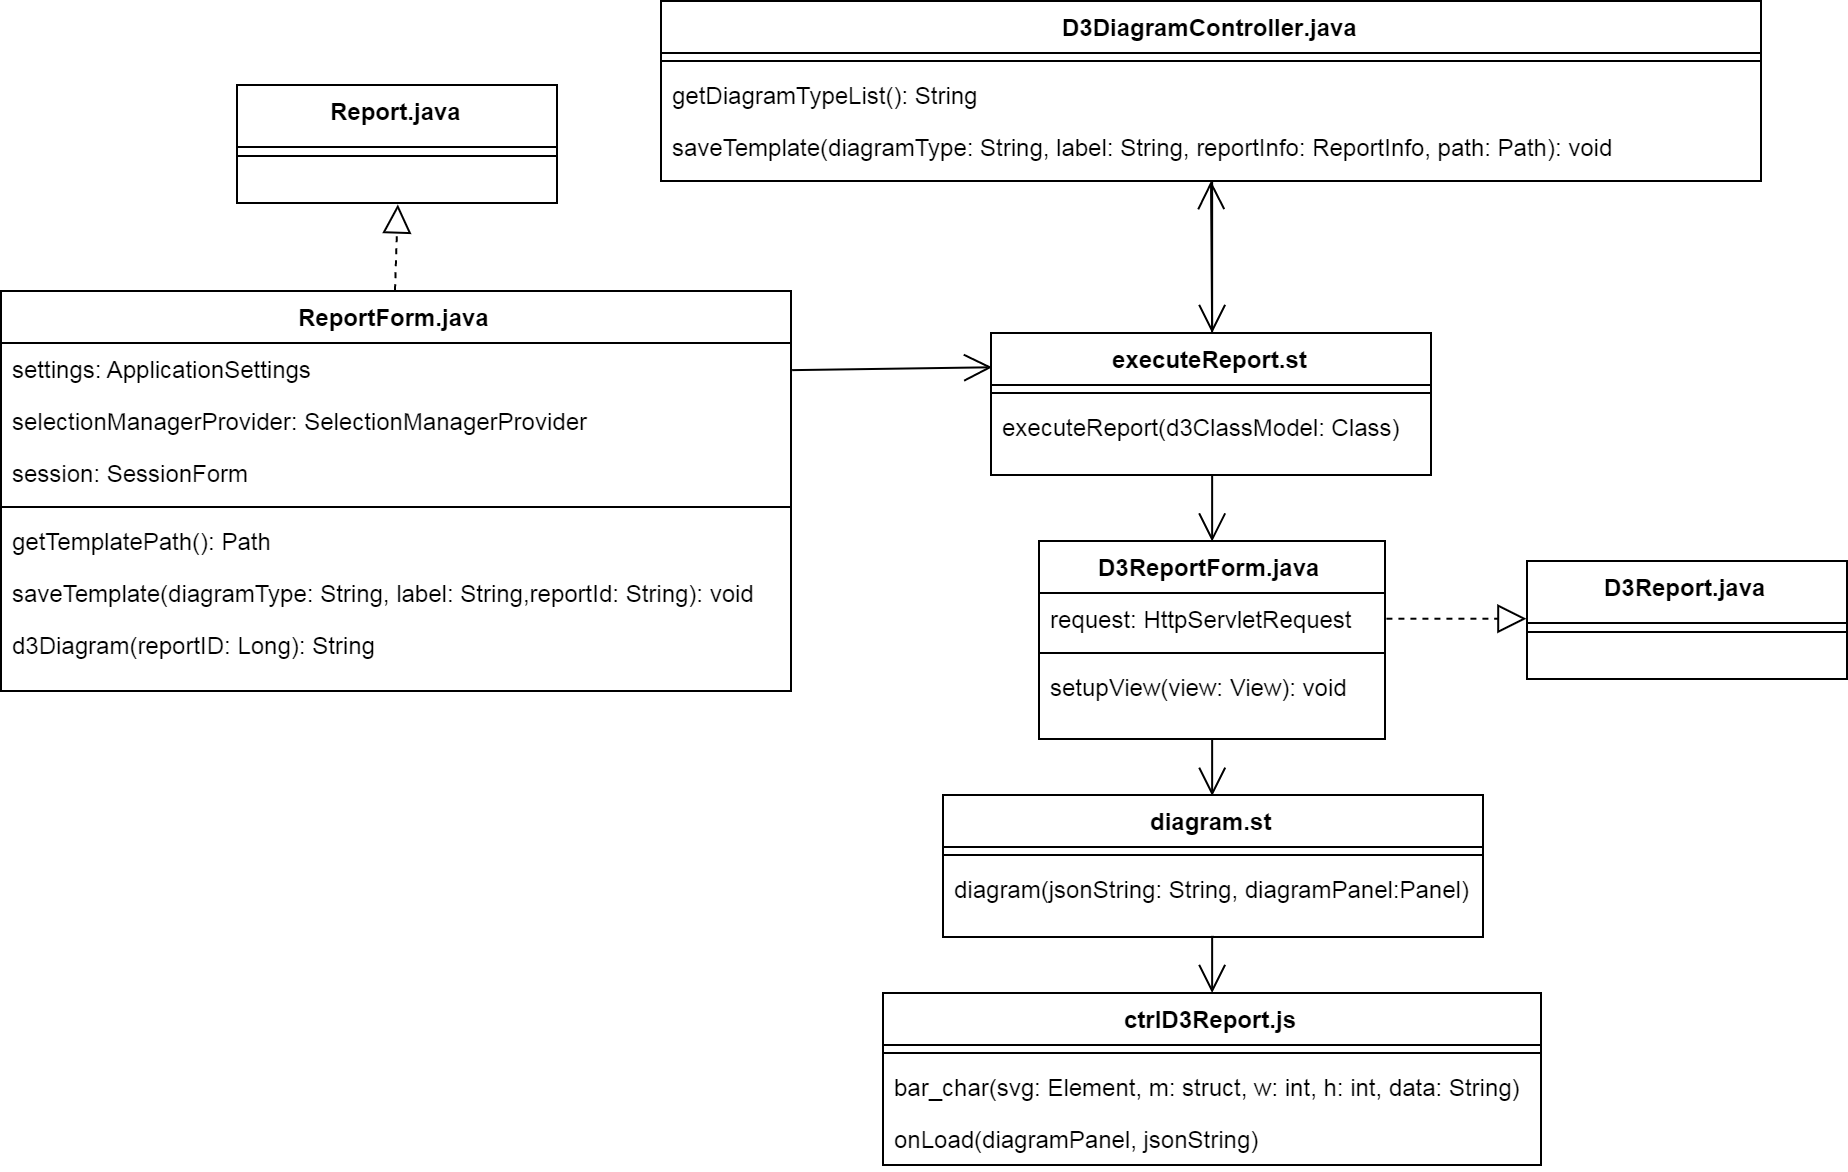
\includegraphics[width=17cm]{./imgs/FullDiagramDesigner.png}}
\caption{UML-диаграмма классов разрабатываемой подсистемы}
\label{umlClassDiagram:ris1}
\end{figure}\par
\begin{figure}[H]
\center{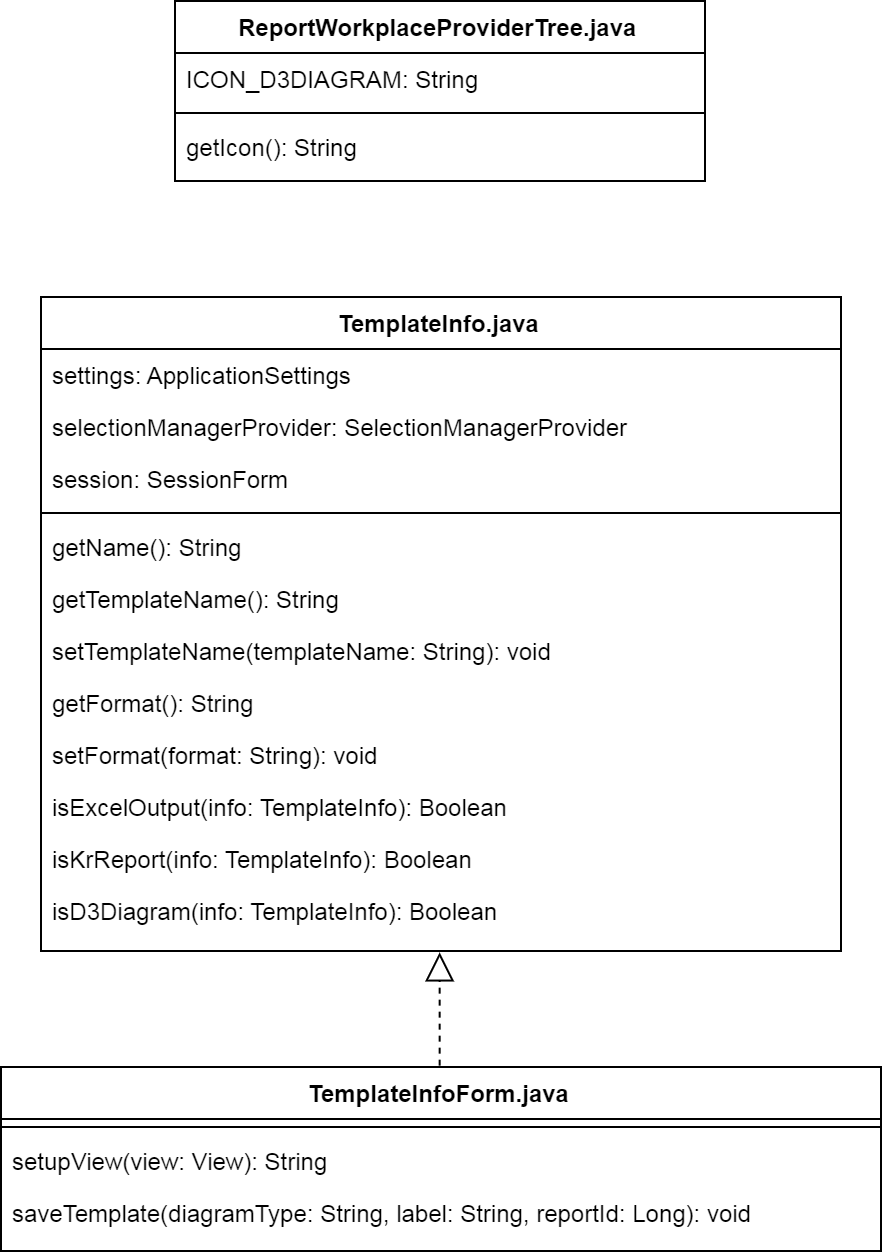
\includegraphics[width=15cm]{./imgs/FullDiagramDesigner_2.png}}
\caption{UML-диаграмма классов разрабатываемой подсистемы}
\label{umlClassDiagram:ris2}
\end{figure}\par
В классе ReportForm происходит вызов скриптового файла executeReport.st, который, в свою очередь, выполняет две основные функции:
\begin{itemize}
\item вызывает метод d3Document класса D3DiagramController, в который передает идентификатор выбранного объекта визуализации. В методе происходит запрос аналитического источника данных из текущей сессии, его обработка в JSON-объект, так же в этом методе происходит обработка шаблона визуализации и пользовательских параметров. После того, как все данные были обработаны, они объединяются в JSON-объект и передаются обратно в executeReport.st.
\item когда executeReport.st получил JSON-объект со всеми необходимыми для построения объекта визуализации данными, он передает их в класс D3ReportForm, в котором происходит передача этого объекта в JavaScript-функцию ctrlD3Report.js, написанную с использованием JavaScript-библиотеки D3.js и выполняющую непосредственное построение объекта визуализации аналитического отчета.
\end{itemize}
В классе D3DiagramController, кроме d3Document, есть еще два метода: getDiagramTypeList и saveTemplate. Первый метод - это геттер для получения списка всех доступных типов диаграмм. Второй метод выполняет сохранение заполненного шаблона визуализации на Редакторе шаблонов. Здесь происзодит обработка полученных с редактора данных и сохранение в ранее созданный файл шаблона с расшинением .template с обработкой возможных исключений и ошибок.\par
Метод ctrlD3Report из JavaScript-файла ctrlD3Report.js написан с использованием JavaScript-библиотеки D3.js и занимается непосредственным построением визуализации. Этот метод имеет четыре внутренних метода:
\begin{itemize}
\item метод onLoad принимает на вход два аргумента: diagramPanel - html-объект в котором будет происходить отображение объекта визуализации и jsonString - JSON-объект со всеми необходимыми для построения объекта визуализации данными (пользовательские параметры, параметры с шаблона визуализации и JSON-объект, полученный при обработке аналитического источника данных. Метод инициализирует начальные параметры, такие как высота и ширина диаграммы, отступы от краев html-объект diagramPanel. Метод так же разделяет данные jsonString на аналитические данные и пользовательские параметры, определяет тип строящейся диаграммы.
\item методы graphic, bar\_char и circle\_char принимают некоторые основные параметры, заданные в методе onLoad, и создают объект визуализации в зависимости от выбранной во время выполнения метода onLiad типа диаграммы.
\end{itemize}
Интерфейс TemplateInfo и его реализация TemplateInfoForm - это классы, которые содержат и предоставляют информацию о шаблонах. Здесь есть следующие методы и поля:
\begin{itemize}
\item метод getName возвращает наименование визуализации;
\item метод getTemplateName возвращает имя файла шаблона (без расширения);
\item метод getFormat возвращает формат шаблона, его расширение, отвечающее за принадлежность шаблона к определенному виду отчета.
\item метод isD3Diagram принимает на вход объект класса TemplateInfo, и возвращает флаг, говорящий о принадлежности объекта к объекту визуализации.
\item поле formats содержит список всех форматов отчетов, доступных в программном комплексе "Web-Исполнение бюджета".
\end{itemize}

\subsection{Программа и методика испытаний}

\subsubsection{Объект испытаний}
Объектом испытаний является подсистема визуализации аналитических отчетов. Данная подсистема предназначена для пользователей программного комплекса "Web-Исполнение Бюджета", чтобы обеспечить им возможность более эффективного анализа данных за счет их визуализации, представления этих данных в графическом представлении, в виде графиков или диаграмм.

\subsubsection{Цель испытаний}
Целью испытаний является проверка корректности работы тех функциональных частей продукта, которые полностью реализованы в процессе  работы.\par

\subsubsection{Требования к программе}
Большинство требований предъявленных к системе являются качественными, а не количественными, вследствие чего их проверка не требует особых усилий. Перечислим требования в таблице (Таблица \ref{tableTreb}).\par
\begin{longtable}[H]{|c|p{0.3\textwidth}|p{0.3\textwidth}|p{0.3\textwidth}|}
  \caption{Требования к программе}
  \label{tableTreb}\\
  \hline
  №  & Требование & Способ оценки & Примечание \\\hline
  \endfirsthead
  1  & Проверка корректности преобразования аналитического источника данных в JSON-объект & Запуск системы в режиме отладки в месте преобразования аналитического источника данных в JSON-объект & Под режимом отладки понимается постановка точки останова в нужном месте и запуск выполнения системы в пошаговом режиме, начиная с установленной точки останова\\
    \multicolumn{4}{l}{}\\\multicolumn{4}{l}{}\\\multicolumn{4}{l}{}\\\multicolumn{4}{l}{}\\
  	\caption*{Продолжение таблицы \ref{tableTreb}} \\\hline
  2  & Проверка корректности создания объекта визуализации в интерфейсе Администратор отчетов & В интерфейса администратор отчетов создать документ, выбрать заполненный шаблон и соответствующий визуализации формат отчета & \\\hline
  3  & Проверка корректности заполнения формы Редактора шаблона (проверка на обязательность заполнения всех полей) & Запустить Редактор шаблона с интерфейса Администратор отчетов и проверить все поля на обязательное заполнение & \\\hline
  4  & Проверка корректности исполнения фрагмента кода, отвечающего за сбор пользовательских параметров & Запуск системы в режиме отладки в месте сбора пользовательских параметров & \\\hline
  5  & Проверка корректности объединения двух JSON-объектов (собранные пользовательские параметры и аналитичский источник данных) & Запуск системы в режиме отладки в месте объединения двух JSON-объектов & \\
  	\multicolumn{4}{l}{}\\\multicolumn{4}{l}{}\\\multicolumn{4}{l}{}\\\multicolumn{4}{l}{}\\
  	\caption*{Окончание таблицы \ref{tableTreb}} \\\hline
  6  & Проверка корректнного отображения визуализации в соответствии с заполненным шаблоном, пользовательскими параметрами и аналитическим источников & Выполнение созданной и заполненной визуализации на интерфейса Отчеты & Имеется в виду выполнение в качестве пользователя, а не системного программиста, то есть нажатие кнопки Выполнить на интерфейса Отчеты\\\hline
\end{longtable}\par

\newpage
\subsubsection{Методика испытаний}
\begin{longtable}[H]{|c|p{0.45\textwidth}|p{0.45\textwidth}|}
  \caption{Методика испытаний}
  \label{tableMetod} \\\hline
  №  & Требование & Способ оценки \\\hline
  \multicolumn{3}{|c|}{Проверка корректности работы подсистемы на web-интерфейсе} \\\hline
  1  & Вводимые данные: создание объекта визуализации на интерфейсе Администратор отчетов & Корректное создание объекта без ошибок \\\hline
  2  & Вводимые данные: создание аналитического источника на интерфейсе Аналитические источники данных & Корректное создание объекта без ошибок \\\hline
  3  & Вводимые данные: добавление созданного аналитического источника во вкладку Источники данных в детализации интерфейса Аналитические источники данных & Корректное добавление объекта на интерфейс \\\hline
  4  & Вводимые данные: создание аналитического источника во вкладке Источники данных в детализации интерфейса Аналитические источники данных & Корректное создание и добавление объекта на интерфейс \\\hline
  \multicolumn{3}{|c|}{Проверка корректности работы подсистемы на стороне сервера} \\\hline
  5  & Вводимые данные: проверка корректности преобразования аналитического источника данных в JSON-объект & JSON-объект с идентичными исходному аналитическому источнику полями \\\hline
  6  & Вводимые данные: проверка корректности исполнения фрагмента кода, отвечающего за сбор пользовательских параметров & Набор java-объектов со значениями соответствующими выбираемым пользовательским параметрам \\
  \multicolumn{3}{l}{}\\\multicolumn{3}{l}{}\\
  \caption*{Окончание таблицы \ref{tableMetod}} \\\hline
  7  & Вводимые данные: проверка корректности объединения двух JSON-объектов (собранные пользовательские параметры и аналитичский источник данных) & JSON-объект с идентичными исходному аналитическому источнику и пользовательским параметрам полями \\\hline
\end{longtable}\par

\newpage
\section{Эксплуатационная документация}

\subsection{Руководство системного программиста}

\subsubsection{Назначение программы}
Подсистема визуализации аналитических отчетов обеспечивает пользователям программного комплекса "Web-Исполнение Бюджета" возможность более эффективного анализа данных за счет их визуализации, представления этих данных в графическом представлении, в виде графиков или диаграмм.

\subsubsection{Условия выполнения программы}
Разрабатываемое программное обеспечение должно функционировать в операционных системах Windows XP(32-bit) / Vista (32- или 64-bit) / Windows 7 (32- или 64-bit).\par
Минимальные требования к техническим характеристикам ПК пользователя:\par
\begin{itemize}
  \item процессор с тактовой частотой не ниже 800 МГц;
  \item объем оперативной памяти (RAM): 4 Гб;
  \item дисковая подсистема с объемом свободной памяти не менее 20 Гб.
\end{itemize}\par
Требования к каналам связи между клиентским устройством и сервером:\par
\begin{itemize}
  \item время прохождения пакета (ping) от клиента до сервера не больше 100 мс;
  \item скорость передачи данных: от 256 Кбит/с при однопользовательской работе, от 1024 Кбит/с для 2-4 пользователей.
\end{itemize}\par
Для функционирования модуля необходима актуальная версия браузера Mozilla Firefox, Yandex Browser или Google Chrome (с поддержкой версии JavaScript ECMAScript 6 и старше[8]). JavaScript-библиотека jQuery версии 3.1 и старше. JavaScript-библиотека D3.js версии 4.8.0 и старше. При использовании ЭП - криптографическое ПО.

\subsubsection{Управление подсистемой}
Подсистема визуализации аналитических отчетов интегрирована в систему "Web-Исполнение бюджета", поэтому для использования подсистемы необходим доступ к системе с правами администратора. Работа системного программиста по управлению подсистемой происходит следующим образом:
\begin{itemize}
	\item Для начала необходимо создать Аналитический источник данных.\par
	Создание аналитического источника начинается с указания наименования аналитического источника (Рисунок \ref{ris3_1}). Далее следует сохранить документ нажатием кнопки "Принять изменения" в виде галочки на верхней панели кнопок. Далее выбрается Идентификатор данных - это модель данных, из которой будет происходить выборка данных. Добавление происходит в детализации интерфейса Аналитические источники данных во вкладке Секции (Рисунок \ref{ris3_2}). Затем в новый аналитический источник добавляются колонки из модели данных, которые будут использоваться при формировании данных для отчета, для этого следует перейти на вкладку Колонки в детализации интерфейса Аналитические источники данных (Рисунок \ref{ris3_3}). После добавления колонок требуется написать события, которые будут отвечать за содержание данных во время подготовки параметров (событие На подготовку параметров), после закачки данных (событие После закачки) после формирования данных, это делается в самом интерфейса, в его заголовочной части (Рисунок \ref{ris3_1}).
\begin{figure}[H]
\center{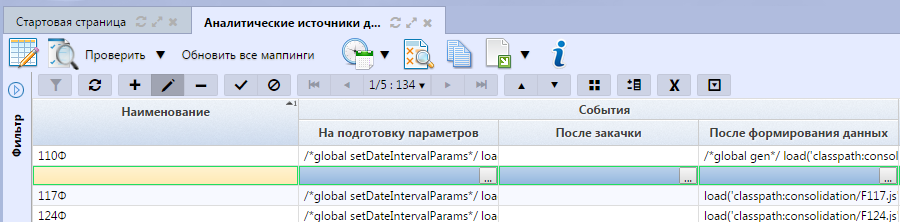
\includegraphics[width=17cm]{./imgs/3_1.png}}
\caption{Интерфейс создания Аналитического источника данных}
\label{ris3_1}
\end{figure}\par
\begin{figure}[H]
\center{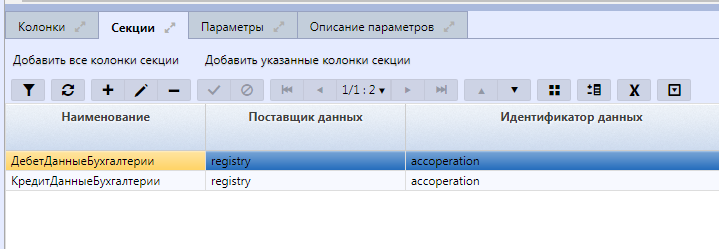
\includegraphics[width=17cm]{./imgs/3_2.png}}
\caption{Вкладка Секции детализации Аналитического источника данных}
\label{ris3_2}
\end{figure}\par
\begin{figure}[H]
\center{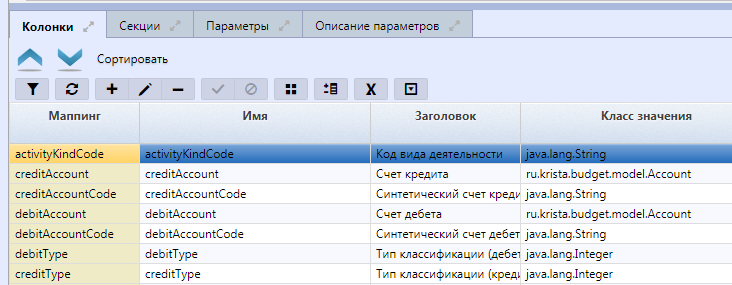
\includegraphics[width=17cm]{./imgs/3_3.png}}
\caption{Вкладка Колонки детализации Аналитического источника}
\label{ris3_3}
\end{figure}\par
	\item Далее создается шаблон визуализации в формате .template. Это делается на интерфейсе Администратор отчетов (Рисунок \ref{ris4_1}). Созданный шаблон можно редактировать на этом же интерфейсе в Редакторе шаблонов (вторая кнопка слева на верхней панель кнопок), где можно выбрать наименование диаграммы, наличие на диаграмме легенды, вид диаграммы и наименование осей (Рисунок \ref{ris5}).
\begin{figure}[H]
\center{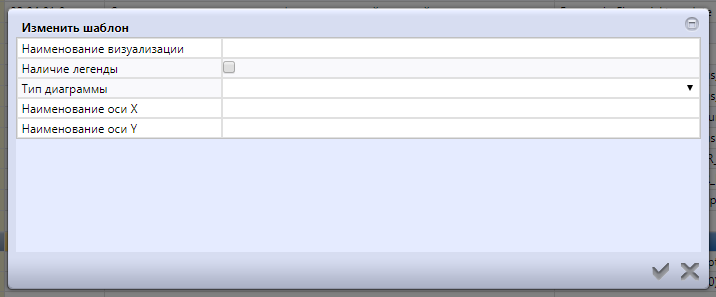
\includegraphics[width=17cm]{./imgs/5.png}}
\caption{Редактор шаблонов на интерфейсе Администратор отчетов}
\label{ris5}
\end{figure}\par
\begin{figure}[H]
\center{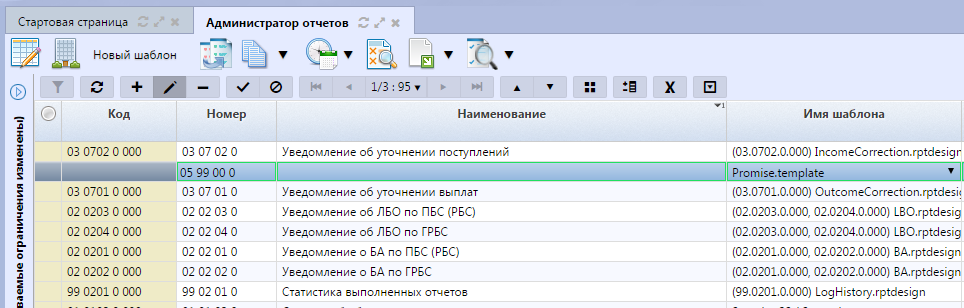
\includegraphics[width=17cm]{./imgs/4_1.png}}
\caption{Интерфейс создания Аналитического отчета}
\label{ris4_1}
\end{figure}\par
    \item Следующим этапом будет создание нового объекта визуализации на интерфейсе Администратор отчетов. Здесь указывается Наименование объекта, выбираются шаблон, созданный ранее и формат отчета (d3\_diagram для объекта визуализации). Далее, в детализации интерфейса Администратор отчетов (Рисунок \ref{ris4_2}), указывается источник данных, созданный ранее, на основании которого будет строится визуализация и указываются нужные параметры визуализации.
\begin{figure}[H]
\center{
\includegraphics[width=12cm]{./imgs/4_2.png}}
\caption{Детализация интерфейса создания Аналитического отчета}
\label{ris4_2}
\end{figure}\par
    \item После создания объекта визуализации его можно выполнить на интерфейсе Отчеты нажав кнопку Выполнить в верхней панели кнопок (Рисунок \ref{ris6}). Здесь, как и на интерфейсе Администратор отчетов можно править шаблон визуализации с помощью Редактора шаблонов.
\begin{figure}[H]
\center{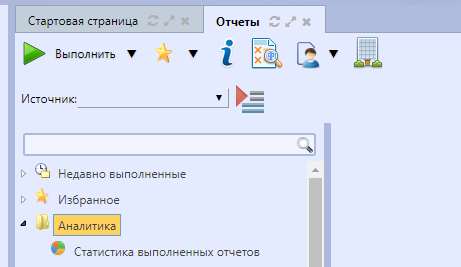
\includegraphics[width=12cm]{./imgs/6.png}}
\caption{Интерфейс Отчеты}
\label{ris6}
\end{figure}\par
\end{itemize}\par

\subsection{Руководство пользователя}

\subsubsection{Назначение программы}
Подсистема визуализации аналитических отчетов обеспечивает пользователям программного комплекса "Web-Исполнение Бюджета" возможностm более эффективного анализа данных за счет их визуализации, представления этих данных в графическом представлении, в виде графиков или диаграмм.

\subsubsection{Условия выполнения программы}
Разрабатываемое программное обеспечение должно функционировать в операционных системах Windows XP(32-bit) / Vista (32- или 64-bit) / Windows 7 (32- или 64-bit).\par
Минимальные требования к техническим характеристикам ПК пользователя:\par
\begin{itemize}
  \item процессор с тактовой частотой не ниже 800 МГц;
  \item объем оперативной памяти (RAM): 4 Гб;
  \item дисковая подсистема с объемом свободной памяти не менее 20 Гб.
\end{itemize}\par
Требования к каналам связи между клиентским устройством и сервером:\par
\begin{itemize}
  \item время прохождения пакета (ping) от клиента до сервера не больше 100~мс;
  \item скорость передачи данных: от 256 Кбит/с при однопользовательской работе, от 1024 Кбит/с для 2-4 пользователей.
\end{itemize}\par
Для функционирования модуля необходима актуальная версия браузера Mozilla Firefox, Yandex Browser или Google Chrome (с поддержкой JavaScript версии ECMAScript 6 и старше). JavaScript-библиотека jQuery версии 3.1 и старше. JavaScript-библиотека D3.js версии 4.8.0 и старше. При использовании ЭП - криптографическое ПО.

\subsubsection{Работа с подсистемой}
Обычные пользователи, которые не имеют прав администратора в системе, имеют доступ только к интерфейсу Отчеты, в котором у них нет прав реактировать шаблон визуализации. Пользователи без прав администратора могут только Выполнять построение визуализации, нажав на кнопку Выпонить в верхней панели кнопок интерфейса Отчеты (Рисунок \ref{ris7}).
\begin{figure}[H]
\center{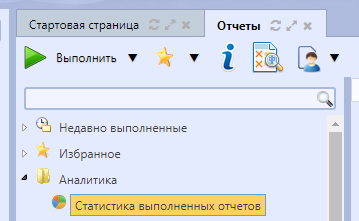
\includegraphics[width=10cm]{./imgs/7.png}}
\caption{Интерфейс Отчеты для пользователя без прав администратора}
\label{ris7}
\end{figure}\par

\newpage
\section{Акт испытаний}

\subsection{Объект испытаний}
Объектом испытаний является подсистема визуализации аналитических отчетов. Данная подсистема предназначена для пользователей программного комплекса "Web-Исполнение Бюджета", чтобы обеспечить им возможность более эффективного анализа данных за счет их визуализации, представления этих данных в графическом представлении, в виде графиков или диаграмм.

\subsection{Цель испытаний}
Целью испытаний является проверка корректности работы тех функциональных частей продукта, которые полностью реализованы в процессе  работы.\par
\subsection{Выводы}
\begin{longtable}[H]{|c|p{0.3\textwidth}|p{0.3\textwidth}|p{0.3\textwidth}|}
  \caption{Результаты испытаний}
  \label{table3} \\\hline
  №  & Требование & Способ оценки & Результат испытаний \\\hline
  \multicolumn{4}{|c|}{Проверка корректности работы подсистемы на web-интерфейсе} \\\hline
  1  & Вводимые данные: создание объекта визуализации на интерфейсе Администратор отчетов & Корректное создание объекта без ошибок & Требование выполнено\\\hline
  2  & Вводимые данные: создание аналитического источника на интерфейсе Аналитические источники данных & Корректное создание объекта без ошибок & Требование выполнено \\
  \multicolumn{4}{l}{}\\
  \caption*{Продолжение таблицы \ref{table3}} \\\hline
  3  & Вводимые данные: добавление созданного аналитического источника во вкладку Источники данных в детализации интерфейса Аналитические источники данных & Корректное добавление объекта на интерфейс & Требование выполнено \\\hline
  4  & Вводимые данные: создание аналитического источника во вкладке Источники данных в детализации интерфейса Аналитические источники данных & Корректное создание и добавление объекта на интерфейс & Требование выполнено \\\hline
  \multicolumn{4}{|c|}{Проверка корректности работы подсистемы на стороне сервера} \\\hline
  5  & Вводимые данные: проверка корректности преобразования аналитического источника данных в JSON-объект & JSON-объект с идентичными исходному аналитическому источнику полями & Требование выполнено \\\hline
  6  & Вводимые данные: проверка корректности исполнения фрагмента кода, отвечающего за сбор пользовательских параметров & Набор java-объектов со значениями соответствующими выбираемым пользовательским параметрам & Требование выполнено \\
  \multicolumn{4}{l}{}\\
  \caption*{Окончание таблицы \ref{table3}} \\\hline
  7  & Вводимые данные: проверка корректности объединения двух JSON-объектов (собранные пользовательские параметры и аналитичский источник данных) & JSON-объект с идентичными исходному аналитическому источнику и пользовательским параметрам полями & Требование выполнено \\\hline
\end{longtable}\par
Испытания подсистемы производили
\begin{itemize}
\item разработчик Ляпушкин Н. А.
\item руководитель выпускной квалификационной работы Маврин С. В.
\end{itemize}\par
Проведя тестирование по всем пунктам методики испытаний, можно сказать, что подсистема работает верно, и удовлетворяет заданным требованиям. Работу можно считать завершенной с положительным результатом.
\vfill
\begin{flushright}
\begin{tabular}{p{.8\textwidth}}
  Студент-дипломник \hrulefill Н. А. Ляпушкин \\
  Руководитель \hrulefill С. В. Маврин
\end{tabular}
\end{flushright}

\newpage
\section{Экономическая часть}

\subsection{Обзор рынка программных продуктов}
Разрабатываемая подсистема визуализации аналитического отчета должна обеспечивать следующую функциональность:\par
\begin{itemize}
  \item возможность преобразовывать аналитический источник данных в удобный для передачи и чтения компонентом визуализации формат;
  \item возможность запрашивать у пользователя параметры визуализации (наименование визуализации, названия осей, тип визуализации);
  \item возможность объединения собранных данных в удобный для передачи и чтения компонентом визуализации формат;
  \item возможность построения объекта визуализации, который должен содержать:
    \begin{itemize}
    	\item наименование визуализации;
        \item легенду, указывающую описание к маркерам данных;
    	\item оси и подписи к ним, если выбрана столбчатая диаграмма или график;
        \item метки осей - категории, которые задают положение конкретных значений в ряде данных;
    \end{itemize}
  \item возможность интеграции объекта визуализации в программный комплекс "Web-Исполнение бюджета".
\end{itemize}\par
Представляемая подсистема создана для узкоспециализированной задачи и использования только в рамках программного продукта "Web-Исполнение бюджета".\par
При изучении рынка специализированного ПО было выявлено, что аналогичные "Web-Исполнению бюджета" системы так же используют подобный функционал. В большинстве этих систем используются комерческие приложения крупных компаний, таких, как Microsoft, Oracle, cluvio и других.\par
Oracle Data Visualization Cloud Service, Microsoft Excel Online и cluvio - это платные коммерческие приложения, которые требуют не разовую оплату продукта, а распространяются по системе подписки.

\subsection{Расчет себестоимости подсистемы}
Расчет себестоимости подсистемы определяется суммированием расходов по следующим пунктам:
\begin{itemize}
\item основная заработная плата;
\item размер социальных отчислений;
\item накладные расходы;
\item материальные затраты;
\item затраты на машинное время;
\item прочие затраты.
\end{itemize}
Далее производится расчет затрат по каждому пункту.\par

\subsubsection{Материальные затраты}
Материальные затраты – вид затрат, образующих себестоимость продукции, и представляющий расходы, осуществленные на приобретение необходимых для производства товаров (выполнения работ, оказания услуг) расходуемых материальных ресурсов.\par
В рамках данной разработки материальные затраты представлены расходами на бумагу, оплата доступа в Интернет и т.п.\par
Расходы на бумагу и прочее можно считать незначительными и пренебречь ими. Доступ в интернет предоставляется по тарифу 550 руб. в месяц. Разработка велась 3 месяца; таким образом, материальные затраты составили 550$\times$3=1650 руб.

\subsubsection{Основная заработная плата}
Размер основной заработной платы (ОЗП) определяется окладом инженера-программиста, количеством разработчиков и сроками разработки:\par
\begin{equation}
\label{form1}
	\text{ОЗП} = \text{СЗП}\times T
\end{equation}\par
где\par
СЗП – стандартная заработная плата (16500 руб.)\par
T – число месяцев разработки (3 месяцев).\par
\begin{equation}
\label{form2}
	\text{ОЗП} = 16500\times 3
\end{equation}\par
Размер  ОЗП = 49500 руб.

\subsubsection{Социальные отчисления}
Отчисления на социальные нужды производятся согласно Федеральному закону №212-ФЗ "О страховых взносах в Пенсионный фонд Российской Федерации, Фонд социального страхования Российской Федерации, Федеральный фонд обязательного медицинского страхования (редакция от 02.04.2014)", который устанавливает следующие тарифы страховых взносов:
\begin{itemize}
  \item Пенсионный фонд Российской Федерации - 22\%;
  \item Фонд социального страхования Российской Федерации - 2,9\%;
  \item Федеральный фонд обязательного медицинского страхования - 5,1\%;
\end{itemize}\par
Суммарный процент социальных отчислений $C_o$ составляет 22\% + 2,9\% + 5,1\%. Соответственно, размер социальных отчислений предриятия на заработную плату равенн:
\begin{equation}
\label{form3}
	\text{О}_\text{соц} = \text{ЗП}\times C_o = \text{ЗП}\times 30\%
\end{equation}\par
Получаем, что $\text{О}_\text{соц}$ = 14850 руб.\par
Сумма затрат предприятия на заявленную заработную плату работников составляет:
\begin{equation}
\label{form4}
	\text{Р}_\text{ЗП}=\text{ЗП}\times(1+C_o)
\end{equation}

\begin{equation}
\label{form5}
	\text{Р}_\text{ЗП}=49500\times(1+0,3)
\end{equation}\par

\subsubsection{Затраты на машинное время}
Расходы на машинное время с учетом наличия 246 дней в году определяются по формуле[9]:\par
\begin{equation}
\label{form6}
	\text{Мвр}=\text{Счмв}\times \text{ВР}_\text{м}
\end{equation}
где $\text{М}_\text{вр}$ – расходы на машинное время, руб.;\par
Счмв – стоимость одного часа машинного времени, руб./час;\par
ВРм – время использования ЭВМ для разработки программного продукта, час.\par
Стоимость одного часа машинного времени можно рассчитать по формуле[9]:\par
\begin{equation}
\label{form7}
	\text{Счмв}=\frac{\text{Цк}}{\text{Ссл}\times 246\times \text{Вэд}}+\text{РЭ}
\end{equation}
где $\text{Ц}_\text{ро}$ – цена рабочего окружения (покупная цена программного и аппаратного обеспечения);\par
Ссл – срок службы компьютера, лет;\par
Вэд – время эксплуатации ЭВМ в день, час;\par
Рэ – эксплуатационные расходы, руб./час.\par
Покупная цена программного и аппаратного обеспечения составляет сумму цены компьютера, цены операционной системы и цены среды разработки[9]:
\begin{equation}
	\text{Ц}_\text{ро} = \text{Ц}_\text{к}+\text{Ц}_\text{OS}+\text{Ц}_\text{ср}
\end{equation}
где $\text{Ц}_\text{ро}$ – цена рабочего окружения;\par
$\text{Ц}_\text{к}$ – цена компьютера с учетом всех комплектующих (35000 руб.);\par
$\text{Ц}_\text{OS}$ – цена операционной системы (9000 руб.);\par
$\text{Ц}_\text{ср}$ – цена среды разработки (840 руб. в месяц $\times$ 3 месяца = 2520 руб.).\par
Эксплуатационные расходы Pэ вычисляются по формуле[9]:\par
\begin{equation}
	\text{Ц}_\text{ро} = 35000+9000+2520=46520
\end{equation}
\begin{equation}
\label{form8}
	\text{Рэ}=\text{Сэ}\times \text{Р}=4\times 0.3\approx 1.2 \text{ руб./час}
\end{equation}
где Сэ – стоимость 1кВт$\times$ч электроэнергии, руб./кВт$\times$ч;\par
Р – суммарная потребляемая мощность вычислительной системы, кВт.\par
Рассчитаем стоимость одного часа машинного времени[9]:\par
\begin{equation}
\label{form9}
	\text{Счмв}=\frac{46520}{8\times 246\times 3}+1.2 = 9,07\text{ руб./час}
\end{equation}\par
Возьмем среднее значение рабочих дней в месяц (21 день), время работы вычислительной машины равно 21$\times$3 = 63 (дня), то есть в часах время использования ЭВМ составит[9]:\par
\begin{equation}
\label{form10}
	\text{ВРм}=63\times 8=288\text{ (ч.)}
\end{equation}
Следовательно, можно найти расходы на машинное время[9]:
\begin{equation}
\label{form11}
	\text{Мвр}=\text{Счмв}\times\text{ВРм}=9,07\times 288 = 2612,16\text{ руб.}
\end{equation}
\subsubsection{Накладные расходы}
В накладных расходах учитываются расходы на управление, коммунальные услуги, аренду помещения. Величина накладных расходов[9] определяется в процентах от основной заработной платы, составляет 30\%, т.е. 14850 руб.:
\begin{equation}
\label{form12}
	\text{Р}_\text{Н}=49500\times 0,3=14850\text{ руб.}
\end{equation}

\subsubsection{Прочие затраты}
Прочие затраты могут включать:
\begin{itemize}
\item командировочные расходы разработчика, связанные с процессом разработки (учитываются по нормативу);
\item коммерческие расходы, связанные с реализацией программного продукта (в размере 2 – 3\% от производственной себестоимости – суммы материальных затрат, заработной платы с отчислениями и стоимости машинного времени);
\item расходы на рекламу.
\end{itemize}\par
При расчете суммы общих затрат будем исходить из того, что командировочные расходы и расходы на рекламу отсутствуют, а величина коммерческих расходов составляет 2,5\% от производственной себестоимости программного продукта:
\begin{equation}
\label{form13}
	\text{ПР}=(\text{МЗ}+\text{ОЗП}+\text{О}_\text{есн}+\text{Мвр}+\text{Р}_\text{Н})\times 0,025
\end{equation}
$$\text{ПР}=(1650+49500+14850+2612,16+14850)\times 0,025=2086,55\text{ руб.}$$

\subsubsection{Определение себестоимости разрабатываемой подсистемы}
Себестоимость разработки программного средства представляет собой сумму затрат по экономическим элементам, приведенным в таблице 1.\par
\begin{table}[H]
\caption{Экономические элементы для расчета $\text{П}_\text{себ}$}
  \begin{tabular}{|c|c|}
  \hline
  Затраты & Сумма, руб. \\\hline
  Материальные затраты & 1650 \\\hline
  Основная заработная плата & 49500 \\\hline
  Социальные отчисления & 14850 \\\hline
  Затраты на машинное время & 2612,16 \\\hline
  Накладные расходы & 14850 \\\hline
  Прочие затраты & 2086,55 \\\hline
  Итог: & 85548,71 \\
  \hline
  \end{tabular}
\end{table}\par
Таким образом, стоимость разработки составила 85548,71 руб.\par

\subsection{Оценка эффекта от продажи подсистемы}

\subsubsection{Расчет прибыли от продажи одной копии подсистемы}
Разрабатываемая подсистема попадает в следующую версию программного комплекса "Web-Исполнения бюджета". На данный момент заказ на неё оформлен 8 заказчиками:\par
\begin{table}[H]
\caption{Заказчики, согласившиеся включить в следющее обновление разработанную подсистему}
  \begin{tabular}{|c|c|}
  \hline
  № & Наименование \\\hline
  1 & Долгопрудный (ФУ) Московская обл. \\\hline
  2 & Ленинский район (ФУ) Московская обл. \\\hline
  3 & Можайский район (ФКУ) Московская обл. \\\hline
  4 & Орехово-Зуево (ФУ ГО) Московская обл. \\\hline
  5 & Подольск (ФУ) Московская обл. \\\hline
  6 & Пушкинский р-н (КФНП) Московская обл. \\\hline
  7 & Фрязино (ФУ) Московская обл. \\\hline
  8 & Электросталь (ФУ) Московская обл. \\\hline
  \end{tabular}
\end{table}\par

Расчет прибыли от продажи одной копии подсистемы осуществляется по следующей формуле[9]:
\begin{equation}
\label{form13}
	\text{П}_\text{ед}=\text{Ц}-\text{НДС}-\frac{\text{З}_\text{р}}{N}
\end{equation}
где $\text{П}_\text{ед}$ - прибыли от продажи одной копии;\par
$\text{Ц}$ - цена одной копии;\par
$\text{НДС}$ - налог на добавленную стоимость;\par
$\text{З}_\text{р}$ - затраты на реализацию;\par
N - количество заказчиков.\par
За цену одной копии возьмем 20\% от себестоимости подсистемы, то есть $85548,71\times 0,2 = 17000$ руб.
Рассчитаем НДС[9]:
\begin{equation}
\label{form14}
	\text{НДС}=\frac{\text{Ц}\times \text{\%НДС}}{100\%+18\%}=\frac{17000\times 18\%}{100\%+18\%}=2609,9 \text{ руб.}
\end{equation}\par
Рассчитаем затраты на реализацию, которые составляют 10\% от себестоимости разработки[9]:
\begin{equation}
\label{form15}
	85548,71\times 0,1 = 8554,87 \text{ руб.}
\end{equation}\par
Таким образом прибыль от продажи одной копии будет составлять:
\begin{equation}
\label{form16}
	\text{П}_\text{ед}=17000-2609,9-\frac{85548,71+8554,87}{8}=2627,15\text{ руб.}
\end{equation}
Затраты на разработку и реализацию составляют 85548,71 и 8554,87 руб. соответственно. Доход от продажи одной копии подсистемы составляет:\par
\begin{equation}
\label{form17}
	\text{Ц}-\text{\%НДС} = 17000-2609,9 = 14390,1 \text{ руб.}
\end{equation}\par
Рассчитаем количество копий, которые необходимо продать для окупаемости затрат:\par
\begin{equation}
\label{form18}
	\frac{85548,71+8554,87}{14390,1}=7 \text{ (копий)}
\end{equation}
После 7 проданных заказчикам копий, дальнейшие продажи будут приносить прибыль.

\subsubsection{Экономический эффект от внедрения подсистемы}
Подсистема визуализации аналитических отчетов позволит пользователям "Web-Исполнение бюджета" сократить в несколько раз время, затрачиваемое на обновление и сбор данных об организациях.\par
Критерием эффективности создания и внедрения новых средств автоматизации является ожидаемый экономический эффект. Он определяется по формуле[9]:\par
\begin{equation}
\label{form19}
	\text{Э}=\text{Э}_\text{р}-\text{Е}_\text{н}\times \text{К}_\text{п}
\end{equation}\par
где $\text{Э}_\text{р}$ - годовая экономия;\par
$\text{Е}_\text{н}$ - нормативный коэффициент (0,15);\par
$\text{К}_\text{п}$ - капитальные затраты на проектирование и внедрение, включая первоначальную стоимость программы.\par
К капитальным затратам необходимо отнести себестоимость подсистемы 85548,71 руб.\par
\begin{equation}
\label{form20}
	\text{Э}_\text{р}=(\text{Р}_\text{1}-\text{Р}_\text{2})+\Delta\text{Р}_\text{п}
\end{equation}\par
Эксплуатационные расходы не снижаются, поэтому при расчете экономии основным показателем будет экономия от повышения производительности труда($\Delta\text{Р}_\text{п}$).\par
Если учитывать среднюю заработную плату сотрудников федеральных органов государственной власти, работающих с программным комплексом "Web-Исполнением бюджета" - 30 000 руб./месяц, то повышение производительности труда $\text{Р}_i$ (\%) определяется по формуле[9]:\par
\begin{equation}
\label{form21}
	\text{Р}_i=(\frac{\Delta T_j}{F_j-\Delta T_j})\times 100\%
\end{equation}\par
где $F_j$ - время, которое планировалось пользователем для выполнения работы j-го вида до внедрения программы;\par
$\Delta T_j$ - экономия времени с применением доработки.\par
Если учесть, что сотрудник федерального органа государственной власти обычно тратит 4 часа в день на анализ табличных отчетов, то в месяц у сотрудника уходит 84 часа. Визуализация аналитического отчета увеличит наглядность табличных данных, поэтому преположим, что сотрудник в день станет тратить 1 час на анализ данных, то есть 21 часа в неделю.\par
Экономия в процентах для подсистемы вычисляется по формуле[9]:
\begin{equation}
\label{form22}
	\text{P}_i=(\frac{63}{84-63})\times 100\%=300\%
\end{equation}\par
Можно сказать, что при использовании доработки сотрудник стал гораздо эффективнее тратить рабочее время, соответственно у него освободилось время на реализацию других задач. Из этого можно сделать вывод, что обеим сторонам будет выгодна данная доработка.

\newpage
\section*{Заключение}
\addcontentsline{toc}{section}{Заключение}
В результате выполнения выпускной квалификационной работы была разработана подсистема визуализации аналитических отчетов.\par
Разработанная подсистема обеспечивает следующую функциональность:\par
\begin{itemize}
  \item преобразовывает аналитический источник данных в удобный для передачи и чтения компонентом визуализации формат;
  \item запрашивает у пользователя параметры визуализации (наименование визуализации, названия осей, тип визуализации);
  \item объединяет собранные данные в удобный для передачи и чтения компонентом визуализации формат;
  \item строит объект визуализации, содержащий:\newline
    	\hspace*{2.5cm} – наименование визуализации;\newline
        \hspace*{2.5cm} – легенду, указывающую описание к маркерам данных;\newline
    	\hspace*{2.5cm} – оси и подписи к ним;\newline
        \hspace*{2.5cm} – метки осей;
  \item возможность интеграции объекта визуализации в программный комплекс "Web-Исполнение бюджета".
\end{itemize}\par
Выполнена поставленная цель по встраиванию подсистемы в программный комплекс автоматизированной системы "Web-Исполнение Бюджета" и поддержке корректной работы в актуальных версиях браузеров Mozilla Firefox, Yandex Browser, Google Chrome. Были улучшены навыки работы с JavaScript-библиотеки D3.JS, улучшены навыки наполнения и разбора JSON-объектов, получены навыки составления технической документации.

\newpage
\section*{Список литературы}
\addcontentsline{toc}{section}{Список литературы}
\begin{enumerate}
\item Общее описание системы ООО НПО Криста [Электронный ресурс]: https://www.krista.ru/files/catalog/ (дата обращения: 12.05.2017)
\item Руководство по JavaScript [Электронный ресурс]: https://developer.mozilla.org/en-US/docs/Web/JavaScript/Reference/ (дата обращения: 07.05.2017)
\item Формат JSON [Электронный ресурс]: https://learn.javascript.ru/json/ (дата обращения: 07.05.2017)
\item Bruce Eckel Thinking in Java, 4th ed.— President, MindView, Inc., 2006.~—~1150~с.
\item Nicl Qi Zhu Data Visualization with D3.js.— PacktPub, 2013. — 332 c.
\item Richard Warburton Java 8 Lambdas.— O'Reilly Media, 2014. — 182 с.
\item Scott Murray Interactive Data Visualization for the Web.— O'Reilly Media, 2013. — 272 с.
\item Ved Antani Mastering JavaScript.— MindView, Inc., 2016. — 250 с.
\item Буч Г., Рамбо Д., Джекобсон А. Язык UML. Руководство пользователя. – М.: ДМК, 2000. — 432 с.
\item "Бюджетный кодекс Российской Федерации" от 31.07.1998 № 145-ФЗ (принят ГД ФС РФ 17.07.1998) (ред. от 24.07.2008).
\item Дэвид Флэнаган JavaScript. Карманный справочник. – М.: Вильямс, 2015. — 320 с.
\item Курс лекции по ООП. Учебное пособие. – Рыбинск: РГАТА, 2008.~—~88~с.
\item Кустова Т. Н., Коновал О.В. Методические рекомендации по технико- экономическому обоснованию дипломных работ студентов специальности 220400 программное обеспечение вычислительной техники и автоматизированных систем. Учебно-методическое пособие. – Рыбинск: РГАТА, 2003. – 39 с.
\item Стив Макконнелл Совершенный код. Мастер-класс. – М.: Русская Редакция, Microsoft Press, 2017. — 896 с.
\item Мартин Фаулер Поделиться: 0 Архитектура корпоративных программных приложений. – М.: Вильямс, 2016. — 544 с.
\end{enumerate}

\newpage
\section*{Приложение А.Исходный код}
\noindent Листинг клиентского скрипта executeReport.st:
\lstinputlisting[language=Java]{executeReport.st}
\noindent Листинг класса D3ReportForm.java:
\lstinputlisting[language=Java]{D3ReportForm.java}
\noindent Листинг скрипта построения визуализации:
\lstinputlisting[language=Java]{ctrlD3Report.js}
\section*{Приложение Б.Пример файла шаблона}
\begin{figure}[H]
\center{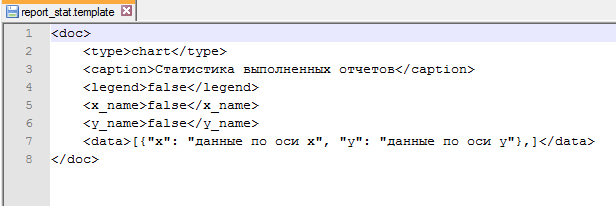
\includegraphics[width=17cm]{./imgs/report_stat.png}}
\label{report_stat}
\end{figure}
\begin{center}
Рисунок Б.1 - Интерфейс создания Аналитического отчета
\end{center}

\end{document}